% Figure 1c (fig:overview): the DISCELL computation graph for one cell i.
% Compile from this directory:  pdflatex fig_model_graph.tex
% build.sh in this directory compiles it and copies the PDF to ../fig_model_graph.pdf
\documentclass[tikz,border=1.5pt]{standalone}
\usepackage{amsmath,amssymb,amsthm,bm,xcolor}
% ---------------------------------------------------------------------------
% Notation and editorial macros for the DISCELL manuscript
% ---------------------------------------------------------------------------
\newcommand{\needsource}{\textcolor{red}{\textbf{[NEEDS A SOURCE]}}}
\newcommand{\todo}[1]{\textcolor{orange}{\textbf{[TODO: #1]}}}
\newcommand{\pending}[1]{\textcolor{violet}{\textbf{[PENDING RUNS: #1]}}}

% operators
\DeclareMathOperator{\sgop}{sg}
\newcommand{\sg}[1]{\sgop\!\left[#1\right]}
\DeclareMathOperator{\KL}{KL}
\DeclareMathOperator{\softmax}{softmax}
\DeclareMathOperator{\Mult}{Multinomial}
\DeclareMathOperator{\Pois}{Poisson}
\DeclareMathOperator{\CE}{CE}
\DeclareMathOperator{\diag}{diag}
\DeclareMathOperator{\logdet}{logdet}
\DeclareMathOperator{\embed}{embed}
\DeclareMathOperator{\onehot}{onehot}
\DeclareMathOperator{\GAT}{GATv2}
\DeclareMathOperator{\I}{I}
\DeclareMathOperator{\E}{\mathbb{E}}
\DeclareMathOperator{\Var}{Var}
\DeclareMathOperator{\corr}{corr}
\DeclareMathOperator{\NMI}{NMI}
\DeclareMathOperator{\simop}{sim}
\newcommand{\att}{\pi}   % attention weight, distinct from the loss weights alpha

% sets and fields
\newcommand{\R}{\mathbb{R}}
\newcommand{\Nat}{\mathbb{N}}
\newcommand{\N}{\mathcal{N}}
\newcommand{\simplex}[1]{\Delta^{#1}}
\newcommand{\nbr}[1]{\mathcal{N}_{#1}}

% vectors
\newcommand{\vx}{\mathbf{x}}
\newcommand{\vy}{\mathbf{y}}
\newcommand{\vz}{\mathbf{z}}
\newcommand{\vw}{\mathbf{w}}
\newcommand{\vc}{\mathbf{c}}
\newcommand{\vv}{\mathbf{v}}
\newcommand{\vu}{\mathbf{u}}
\newcommand{\vB}{\mathbf{B}}
\newcommand{\vI}{\mathbf{I}}
\newcommand{\vPhi}{\boldsymbol{\Phi}}
\newcommand{\vrho}{\boldsymbol{\rho}}
\newcommand{\rhobar}{\bar{\boldsymbol{\rho}}}
\newcommand{\vp}{\mathbf{p}}
\newcommand{\vmu}{\boldsymbol{\mu}}
\newcommand{\vsigma}{\boldsymbol{\sigma}}
\newcommand{\wbreve}{\breve{\mathbf{w}}}
\newcommand{\ybar}{\bar{\mathbf{y}}}
\newcommand{\Phibar}{\bar{\boldsymbol{\Phi}}}
\newcommand{\Sig}{\boldsymbol{\Sigma}}
\newcommand{\Sighat}{\hat{\boldsymbol{\Sigma}}}
\newcommand{\lbar}{\bar{\ell}}
\newcommand{\ephi}{e^{\Phi}}
\newcommand{\Ephi}{E_{\Phi}}
\newcommand{\dz}{d_z}
\newcommand{\dw}{d_w}
\newcommand{\dPhi}{d_{\Phi}}
\newcommand{\alphaz}{\alpha_z}
\newcommand{\alphaw}{\alpha_w}
\newcommand{\alphaa}{\alpha_a}
\newcommand{\mpsi}{m_{\psi}}
\newcommand{\Pen}{\mathrm{Pen}}
\newcommand{\Adv}{\mathrm{Adv}}
\newcommand{\dCE}{\Delta\!\CE}
\newcommand{\um}{\,\mu\text{m}}

\newtheorem{proposition}{Proposition}
\newtheorem{remark}{Remark}

\usetikzlibrary{arrows.meta,calc,positioning}

% --- palette: identical roles to figures/src/style.py -----------------------
\definecolor{blue}{HTML}{2A78D6}  \definecolor{bluefill}{HTML}{E3EEFC}
\definecolor{aqua}{HTML}{1BAF7A}  \definecolor{aquafill}{HTML}{E1F4EC}
\definecolor{ink}{HTML}{0B0B0B}   \definecolor{ink2}{HTML}{52514E}
\definecolor{muted}{HTML}{898781} \definecolor{ghost}{HTML}{F1F0EC}
\definecolor{celledge}{HTML}{A9A79F}

\tikzset{
  every node/.style={font=\footnotesize, text=ink, inner sep=2.2pt},
  net/.style={draw=blue, line width=0.6pt, fill=bluefill, rounded corners=2pt,
              minimum height=6.2mm, minimum width=14mm, align=center},
  data/.style={draw=celledge, line width=0.5pt, fill=ghost, rounded corners=1pt,
               minimum height=6.2mm, align=center},
  comp/.style={draw=ink2, line width=0.5pt, fill=white, minimum height=6.2mm, minimum width=7.2mm, align=center},
  lat/.style={draw=ink, line width=0.6pt, fill=white, circle, minimum size=7.2mm, inner sep=0.5pt},
  adv/.style={draw=aqua, line width=0.6pt, fill=aquafill, rounded corners=2pt,
              minimum height=6.2mm, align=center},
  probe/.style={draw=ink2, line width=0.5pt, dashed, fill=white, rounded corners=2pt,
                minimum height=6.2mm, align=center},
  arr/.style={-{Stealth[length=3.6pt,width=3pt]}, draw=ink2, line width=0.55pt},
  darr/.style={arr, dashed},
  lab/.style={font=\scriptsize, text=ink2, inner sep=1pt},
  lane/.style={font=\scriptsize\itshape, text=muted, anchor=west},
}

\begin{document}
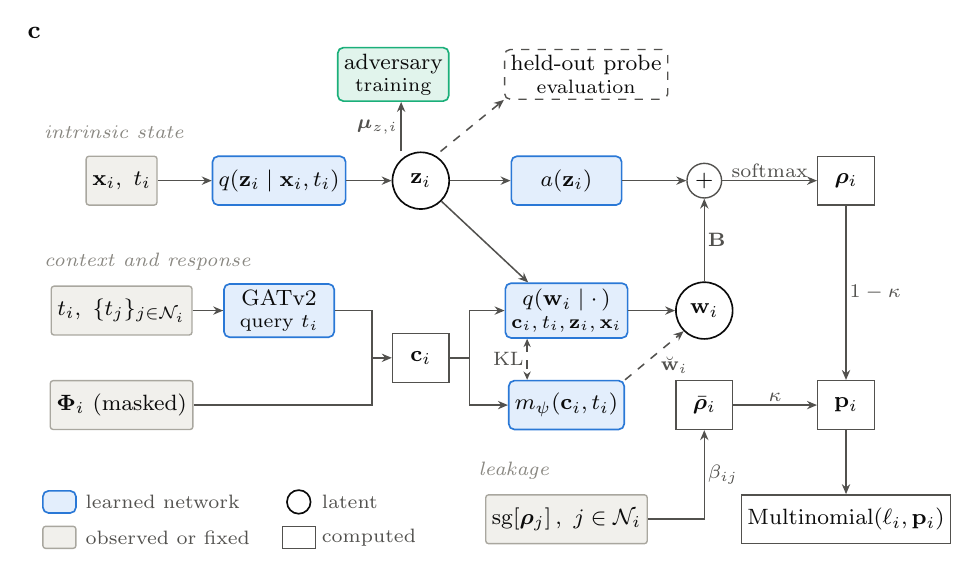
\begin{tikzpicture}
% ---- grid (cm) --------------------------------------------------------------
\def\xA{0.95} \def\xB{2.95} \def\xC{4.75} \def\xD{6.6} \def\xE{8.35} \def\xF{10.15}
\def\rV{6.35} \def\rT{5.0} \def\rM{3.35} \def\rP{2.15} \def\rL{0.7}
\def\rC{2.75}   % c_i sits between the posterior and prior rows

\node[font=\small\bfseries, anchor=north west, inner sep=0pt] at (-0.25, 6.95) {c};
% ---- lane labels --------------------------------------------------------------
\node[lane] at (-0.12, \rT+0.62) {intrinsic state};
\node[lane] at (-0.12, \rM+0.62) {context and response};
\node[lane] at (\xD-1.2, \rL+0.62) {leakage};

% ---- inputs (data) ------------------------------------------------------------
\node[data] (x)   at (\xA, \rT) {$\vx_i,\ t_i$};
\node[data] (t)   at (\xA, \rM) {$t_i,\ \{t_j\}_{j\in\nbr{i}}$};
\node[data] (phi) at (\xA, \rP) {$\vPhi_i$ (masked)};

% ---- intrinsic lane -----------------------------------------------------------
\node[net] (encz) at (\xB, \rT) {$q(\vz_i \mid \vx_i, t_i)$};
\node[lat] (z)    at (\xC, \rT) {$\vz_i$};
\node[net] (dec)  at (\xD, \rT) {$a(\vz_i)$};
\node[draw=ink2, line width=0.5pt, circle, inner sep=0.6pt, minimum size=4.4mm] (plus) at (\xE, \rT) {$+$};
\node[comp] (rho) at (\xF, \rT) {$\vrho_i$};

% ---- context / response lane --------------------------------------------------
\node[net] (gat)  at (\xB, \rM) {$\GAT$\\[-1.5pt]{\scriptsize query $t_i$}};
\node[comp] (c)   at (\xC, \rC) {$\vc_i$};
\node[net] (qw)   at (\xD, \rM) {$q(\vw_i \mid \cdot\,)$\\[-1.5pt]{\scriptsize $\vc_i, t_i, \vz_i, \vx_i$}};
\node[net] (pw)   at (\xD, \rP) {$\mpsi(\vc_i, t_i)$};
\node[lat] (w)    at (\xE, \rM) {$\vw_i$};

% ---- leakage and likelihood ---------------------------------------------------
\node[data] (nb)   at (\xD, \rL) {$\sg{\vrho_j},\ j\in\nbr{i}$};
\node[comp] (rbar) at (\xE, \rP) {$\rhobar_i$};
\node[comp] (p)    at (\xF, \rP) {$\vp_i$};
\node[comp] (lik)  at (\xF, \rL) {$\Mult(\ell_i, \vp_i)$};

% ---- invariance, reading the posterior mean of z ------------------------------
\node[adv]   (adv)   at (\xC-0.35, \rV) {adversary\\[-1.5pt]{\scriptsize training}};
\node[probe] (probe) at (\xD+0.25, \rV) {held-out probe\\[-1.5pt]{\scriptsize evaluation}};

% ---- edges: intrinsic ---------------------------------------------------------
\draw[arr] (x) -- (encz);
\draw[arr] (encz) -- (z);
\draw[arr] (z) -- (dec);
\draw[arr] (dec) -- (plus);
\draw[arr] (plus) -- node[lab, above] {softmax} (rho);

% ---- edges: context, response -------------------------------------------------
\coordinate (J) at (\xC-0.62, \rC);   % concatenation into c
\coordinate (S) at (\xC+0.62, \rC);   % c feeds posterior and prior
\draw[draw=ink2, line width=0.55pt] (t) -- (gat);
\draw[arr] (t) -- (gat);
\draw[draw=ink2, line width=0.55pt] (gat.east) -| (J);
\draw[draw=ink2, line width=0.55pt] (phi.east) -| (J);
\draw[arr] (J) -- (c.west);
\draw[draw=ink2, line width=0.55pt] (c.east) -- (S);
\draw[arr] (S) |- (qw.west);
\draw[arr] (S) |- (pw.west);
\draw[arr] (z.south east) -- ([xshift=3mm]qw.north west);
\draw[arr] (qw) -- (w);
\draw[arr] (w) -- node[lab, right] {$\vB$} (plus);
\draw[{Stealth[length=3pt,width=2.6pt]}-{Stealth[length=3pt,width=2.6pt]}, draw=ink2, line width=0.5pt, dashed]
     ([xshift=-5mm]qw.south) -- node[lab, left] {$\KL$} ([xshift=-5mm]pw.north);
\draw[darr] (pw.north east) -- node[lab, below right, pos=0.55] {$\wbreve_i$} (w.south west);

% ---- edges: leakage, likelihood -----------------------------------------------
\draw[arr] (nb.east) -| node[lab, pos=0.75, right] {$\beta_{ij}$} (rbar.south);
\draw[arr] (rbar) -- node[lab, above] {$\kappa$} (p);
\draw[arr] (rho) -- node[lab, right] {$1-\kappa$} (p);
\draw[arr] (p) -- (lik);

% ---- edges: invariance --------------------------------------------------------
\draw[arr] ([xshift=-2.5mm]z.north) -- node[lab, left] {$\vmu_{z,i}$} ([xshift=-2.5mm]z.north |- adv.south);
\draw[darr] ([xshift=2.5mm]z.north) -- (probe.south west);

% ---- key ----------------------------------------------------------------------
\begin{scope}[shift={(-0.05, 0.92)}, every node/.style={font=\scriptsize, text=ink2, inner sep=1pt}]
  \node[net, minimum width=4.2mm, minimum height=2.8mm, inner sep=0pt] at (0.21, 0) {};
  \node[anchor=west] at (0.5, 0) {learned network};
  \node[lat, minimum size=3.0mm] at (3.25, 0) {};
  \node[anchor=west] at (3.5, 0) {latent};
  \node[data, minimum width=4.2mm, minimum height=2.8mm, inner sep=0pt] at (0.21, -0.45) {};
  \node[anchor=west] at (0.5, -0.45) {observed or fixed};
  \node[comp, minimum width=4.2mm, minimum height=2.8mm, inner sep=0pt] at (3.25, -0.45) {};
  \node[anchor=west] at (3.5, -0.45) {computed};
\end{scope}
\end{tikzpicture}
\end{document}
